% 图 3(a)：李雅普诺夫等值线与轨迹（精确二维示意）
\documentclass[border=6pt]{standalone}
% 四张示意图共用的字体、颜色与 TikZ 设置
\usepackage{fontspec}
\usepackage{xeCJK}
\setmainfont{TeX Gyre Pagella}
\setCJKmainfont{Noto Serif CJK SC}[AutoFakeSlant=0.15]
\usepackage{unicode-math}
\setmathfont{TeX Gyre Pagella Math}
\usepackage{amsmath}
\usepackage{tikz}
\usetikzlibrary{arrows.meta, positioning, calc, decorations.markings, backgrounds, fit, shapes.geometric}

\definecolor{navy}{HTML}{1E3A8A}
\definecolor{teal}{HTML}{0F766E}
\definecolor{amber}{HTML}{B45309}
\definecolor{softblue}{HTML}{EFF6FF}
\definecolor{softteal}{HTML}{F0FDFA}
\definecolor{softamber}{HTML}{FFFBEB}
\definecolor{border}{HTML}{CBD5E1}
\definecolor{graytext}{HTML}{5B6673}
\definecolor{redalert}{HTML}{991B1B}

\tikzset{
  >=Latex,
  every node/.style={font=\small},
  block/.style={draw=navy, thick, rounded corners=3pt, fill=softblue, align=center},
  bus/.style={thick, graytext},
}

\begin{document}
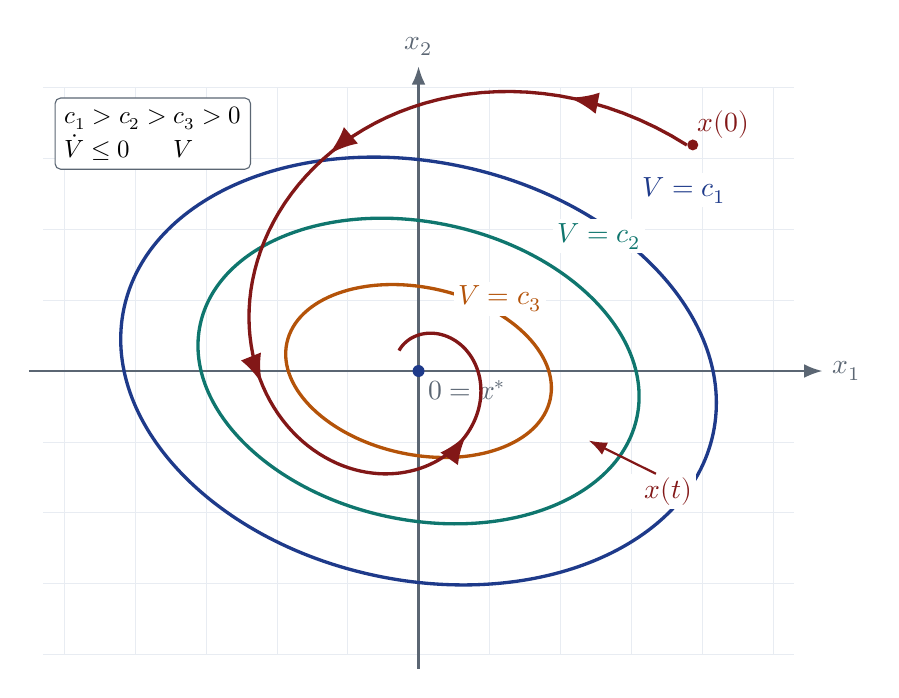
\begin{tikzpicture}[x=1cm,y=1cm,scale=0.90,every node/.style={font=\normalsize}]
  % 网格
  \draw[step=1cm, border!45, very thin] (-5.3,-4.0) grid (5.3,4.0);

  % 坐标轴
  \draw[->, thick, graytext] (-5.5,0) -- (5.7,0) node[right] {$x_1$};
  \draw[->, thick, graytext] (0,-4.2) -- (0,4.3) node[above] {$x_2$};
  \node[below right, text=graytext] at (0,0) {$0=x^\ast$};

  % 等值线 V=c1,c2,c3（c1>c2>c3>0）
  \draw[very thick, navy, rotate around={-12:(0,0)}] (0,0) ellipse (4.25 and 2.95);
  \draw[very thick, teal, rotate around={-12:(0,0)}] (0,0) ellipse (3.15 and 2.10);
  \draw[very thick, amber, rotate around={-12:(0,0)}] (0,0) ellipse (1.90 and 1.18);

  % 等值线标签
  \node[navy, fill=white, inner sep=1.5pt] at (3.75,2.55) {$V=c_1$};
  \node[teal, fill=white, inner sep=1.5pt] at (2.55,1.90) {$V=c_2$};
  \node[amber, fill=white, inner sep=1.5pt] at (1.15,1.02) {$V=c_3$};

  % 轨迹：从外层外部螺旋进入内层
  \draw[very thick, redalert!85!black,
        postaction={decorate},
        decoration={markings,
          mark=at position 0.12 with {\arrow[scale=1.25]{>}},
          mark=at position 0.36 with {\arrow[scale=1.25]{>}},
          mark=at position 0.60 with {\arrow[scale=1.25]{>}},
          mark=at position 0.84 with {\arrow[scale=1.25]{>}}}]
    plot[domain=0:3.6, samples=160]
      ({4.95*exp(-0.70*\x)*cos(deg(0.70+2.20*\x))},
       {4.95*exp(-0.70*\x)*sin(deg(0.70+2.20*\x))});

  % 起点与轨迹标签
  \fill[redalert!85!black] (3.87,3.19) circle (2.2pt);
  \node[redalert!85!black, above right] at (3.80,3.15) {$x(0)$};
  \node[redalert!85!black, fill=white, inner sep=1.5pt] at (3.35,-1.70) {轨迹 $x(t)$};
  \draw[->, thick, redalert!85!black] (3.35,-1.45) -- (2.40,-0.98);

  % 读图辅助：能量下降方向
  \node[draw=graytext, rounded corners=2pt, fill=white, align=left, font=\small]
    at (-3.75,3.35) {$c_1>c_2>c_3>0$\\[1pt]$\dot V\le 0$：箭头指向 $V$ 更小的内层};

  % 原点小圆
  \fill[navy] (0,0) circle (2.4pt);
\end{tikzpicture}
\end{document}
